% !TEX root = template.tex

\section{Introduction}
\label{sec:introduction}
%Intro is here. Points to remember:
%\begin{itemize}
%	\item General short intro: why is this an interesting problem?
%	\item Go on more specifically hinting at what I have done;
%	\item Paper contributions: what is the problem, relevance, approach, value, applicability.
%	\item overview of the structure of the paper..
%	\item stay coincise: try to stay inside one page/one half
	
The Keyword Spotting (KWS) task consists in the detection of a certain predetermined set of keywords from a stream of user utterances. In recent years, this problem has become increasingly popular and, with the rapid development of mobile devices, it is now playing an important role in human-computer interaction, as well as encouraging the adoption of hands-free interfaces for a wide variety of use cases, that can range from \say{smart home} devices like Amazon Alexa, to virtual assistants such as Apple's Siri or Google Assistant. KWS systems are typically required to continuously listen to user inputs on mobile devices, which are highly constrained in their memory and compute capabilities: this restriction has encouraged the development of systems able to achieve highly accurate results but still maintaining a small memory and computational footprint.
%KWS systems play a complementary role with respect to more complex, cloud based speech recognition services: indeed, their are required to run on local devices and are often used to initiate interactions by pronouncing the correct keyword. For this reason the research in KWS typically focuses on a tradeoff between highly precise predictions and small memory/computational footprint.

At present, Deep Learning (DL) techniques represent the state of the art approach for the KWS problem and have proved to give good results on the tradeoff between model lightness and model performance \cite{dnns2014chen} \cite{convnns2015sainath} \cite{streamingkws2020Rybakov}. In the literature, a lot of DL models have been presented, ranging from simple fully connected feed forward networks \cite{dnns2014chen}, to both shallow and very deep Convolutional Neural Networks (CNN) \cite{deepreslearning2018tang} \cite{convnns2015sainath}
\cite{mittermaier2020small} \cite{choi2019temporal}. Especially in recent years, mostly thanks to the work by Vaswani et al.~\cite{attentionisall2017vaswani}, interest towards attention-based architectures has grown dramatically. Indeed, recent works in machine learning have shown that models incorporating attention are able to provide groundbreaking results in a wide variety of domains \cite{vit2020Dosovitskiy} \cite{touvron2021training} \cite{gulati2020conformer} \cite{kumar2021colorization} \cite{Devlin2019BERTPO}. Another charming feature of attention-based systems is their inherent interpretability: by visualizing the attention weights, one can directly see to which part of a specific input the model was paying attention when performing inference tasks. Indeed, Explainable AI (XAI) is quickly becoming an hot topic in modern machine learning research, and the development of models capable of giving some sort of explanation for their predictions  will in time become more and more desirable, if not required \cite{gdpr2017}.

Motivated by those increasing trends, in this work we first give a review of the existing applications of the attention mechanism for the KWS task; then, we propose different variations of an hybrid based on attention, first introduced by de Andreade et al. \cite{attention2018andreade}; this is done mostly to harness the importance of each block in the original model, and to explore new model architectures with relatively small memory footprint in order to obtain better performances. We refer to this baseline as Att-RNN. We summarize the proposed contributions as follows:
\begin{itemize}
	\item We explore variations of the Attention layer: primarily, use more query vectors\footnote{In this work, we use the \textit{query, key, values} terminology introduced in \cite{attentionisall2017vaswani}.} instead of a single one: we call this model SQAtt-RNN. 
	\item We replace the Attention layer with a Multi Head Attention layer \cite{attentionisall2017vaswani}, and explore how model performance changes by varying number of heads.
	\item We explore the role of the convolutional part of Att-RNN, by both removing it and enhancing it with a more complex architecture based on residual layers;
	\item We compare the performances of each proposed model also in terms of the number of parameters.
	
\end{itemize}
Figure \ref{fig:models_overview} shows a representation of the Att-RNN and one of the proposed models SQAtt-RNN. The other architectures will be described in detail later, but can be easily obtained by modifying single blocks starting from those two.

\begin{figure*}
	\centering
	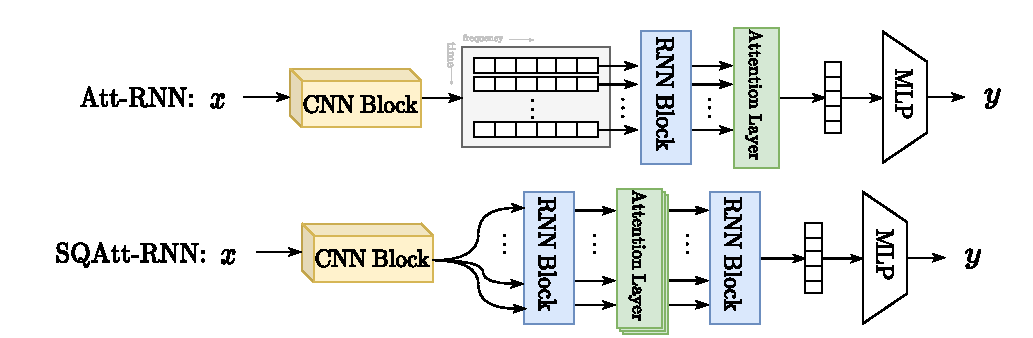
\includegraphics[width=\linewidth]{imgs/models_overview.pdf}
	\caption{Overview of Att-RNN model (baseline) and SQAtt-RNN. The input $x$ is a matrix, where the $i$-th row is the vector of MFCCs computed for the $i$-th time frame. In both models, the CNN block outputs an image where the number of timesteps is preserved: feature vectors at each timestep are used as the input sequence for the RNN block. In the Att-RNN model, the attention layer returns a single context vector which is used for classification. In SQAtt-RNN, we use the whole sequence coming from the RNN block as query vectors: this results in a new sequence which is supposed to be a representation of the previous one. One last Bidirectional RNN layer scans the sequence and returns a single output vector, which is used for classification.}
	\label{fig:models_overview}
\end{figure*}


%\MR{We explore the role of filter size for the convolutional block, to understand if vocal features can be extracted mostly from time or frequency domain.} We also propose some small adjustment to the attention layer and compare the performances with the more modern variant presented in \cite{streamingkws2020Rybakov}. We also examine the Keyword Transformer \cite{kwtransformer2021berg}, a recent architecture that exploits the strength of Transformers in a similar fashion to Vision Transformers \cite{vit2020Dosovitskiy}.

%one of the most explored classes of models is CNNs \cite{deepreslearning2018tang} \cite{convnns2015sainath} \cite{mittermaier2020small} \cite{choi2019temporal}, which are able to capture audio features both in the time and frequency domain, both from spectral and raw audio data. 

